% !TeX root = 场论与凝聚态.tex

The ``microscopic free energy''\footnote{The Mellin transformation of $F$ of variable $\beta$.} will be modified to
\begin{figure}[h]
    \centering
    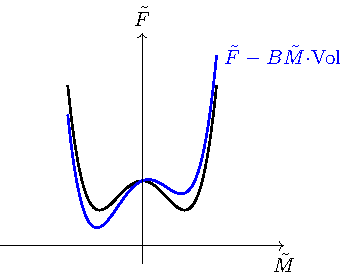
\includegraphics{figures/free_energy_in_external_field.pdf}
    \caption{free energy in external field}
\end{figure}
\begin{equation}
  \tilde{F} = \tilde{F} - B \tilde{M} \cdot \text{Vol}.
\end{equation}
and we have 
\begin{equation}
    \mathcal{Z}\left( B \right)  = \mathrm{e}^{- \frac{F\left( B \right)}{T}} = \int_{-\infty}^{\infty} \mathrm{d}\tilde{M} \, \mathrm{e}^{-\frac{1}{T} \left( \tilde{F} - B \tilde{M} \cdot \text{Vol} \right) } ,
\end{equation}
which is dominated by the double well in $\tilde{F}$.
Meanwhile, we have the relation
\begin{equation}
    M = \frac{1}{\text{Vol}} \frac{\partial F}{\partial B} = \frac{1}{\mathcal{Z}} \frac{\partial \mathcal{Z}}{\partial B} = \left< \tilde{M} \right> 
\end{equation}
and
\begin{equation}
  \chi = \frac{\partial M}{\partial B} = \frac{1}{\mathcal{Z}} \frac{\partial^2 \mathcal{Z}}{\partial B^2} - \frac{1}{\mathcal{Z}^{2}} \frac{\partial \mathcal{Z}}{\partial B} \frac{\partial \mathcal{Z}}{\partial B} = \left< M^{2} \right> - \left< M \right>^{2}
\end{equation}
It can be seen that there's some relation between long range correlation and spontaneous symmetry broken.

\subsection{Long Range Correlation and SSB in Ising Model}

The Hamiltonian of this model is
\begin{equation}
  \begin{gathered}
  H_{\text{classical}} = \sum_{\text{link $l=\langle v\,v' \rangle$}} (-J) \sigma _{v}^{z} \sigma _{v'}^{z}
  \\
  H_{\text{quantum}} = \sum_{\text{vertex $v$}} (-h) \sigma _{v}^{x}+ H_{\text{classical}}
  \end{gathered}
\end{equation}
in which $h$ and $-h$ are equivalent for the $\mathbb{Z}_2$ global symmetry. The corresponding flip operator is
\begin{equation}
  \prod{v} \sigma _{v}^{x}. \quad \text{(one for each part of the space)}
\end{equation}
Note that we doesn't need to flip all spins as our basis spacetime may consist separate parts which do not interact with each other.
The $\mathbb{Z}_2$ symmetry broken term in this model would be $- \sum_{v} B \sigma _{v}^{z}$, and our order parameter is $\sigma _{v}^{z}$.
\begin{itemize}
  \item $H_{\text{quantum}}$ in $d+1$ spacetime can b mapped to $H_{\text{classical}}$ in $d'=d+1$ space, but anisotropic $\tilde{J}_{d}\neq \tilde{J}_{\tau }$.
\end{itemize}

Now let us investigate this system through its partition function
\begin{equation}
  \mathcal{Z} = \left( \prod{v} \sum_{x=\pm 1}  \right)\mathrm{e}^{-\frac{E}{T}}
\end{equation}
where $E = \sum_{l} (-J) s_v s_{v'} - \sum_{v} B_v s_v$. 

Derivations of $\mathcal{Z}$'s logarithm gives statistic observables
\begin{equation}
  M = \frac{1}{\text{Vol}} \frac{\partial F}{\partial B} = \frac{\left( \prod_{v} \sum_{s_v = \pm 1}  \right) s_{v_0} \mathrm{e}^{-\frac{E}{T}}}{\mathcal{Z}} = \langle s_{u_0}\rangle
\end{equation}
and
\begin{equation}
  \begin{aligned}
    \chi = \left. \frac{\partial M}{\partial B} \right|_{B=0} 
    & = \frac{1}{T} \sum_{v_1} \left( \langle s_{v_0} s_{v_1} \rangle - \langle s_{v_0}\rangle \langle s_{v_1}\rangle \right)_{B=0} \\
    & = \frac{1}{T} \sum_{v_1} \langle s_{v_0} s_{v_1}\rangle
  \end{aligned}
\end{equation}

% TODO 
